% ===========================================================================
\section{Evaluation}
\label{sec:evaluation}
% ===========================================================================

The evaluation answers four questions: (Q1)~does the pipeline produce a
verifiable, on-chain-anchored evidence record from a real print job;
(Q2)~does physical adherence propagate into a meaningful reputation
update; (Q3)~is tampering with stored evidence detected; (Q4)~what are
the bridge's latency and storage costs.  All four are answered with
measured data from \textbf{five real print jobs} on the Ender-3 testbed,
spanning \textbf{three geometries} (a complex 5\,MB part, a calibration
cube, and a functional mounting bracket) and \textbf{three outcome types}
(completed, cancelled, and a deliberately injected thermal anomaly).
Table~\ref{tab:runs} summarizes the runs; the subsections that follow
walk through a detailed case study, the controlled anomaly comparison,
reputation propagation, tamper detection, and the cost measurements.

\begin{table*}[t]
\centering
\caption{The five real print jobs: three geometries, three outcome types.
All bundles verify (Ed25519 signature and ledger-hash check) and all carry
\icode{compliance}~$=1.0$ (executed G-code hash equals the certified
design).  \icode{q}/\icode{c}/\icode{d} are the assessment dimensions of
Eq.~\eqref{eq:rating}; canonical size is the off-chain signed bundle, whose
on-chain footprint is a constant 369\,B regardless of bundle size.}
\label{tab:runs}
\small
\begin{tabular}{lllccccrrr}
\toprule
Run & Geometry & Outcome & \icode{q} & \icode{c} & \icode{d} & rating $r$
  & samples & canon.\ B & on-chain B \\
\midrule
\icode{f4u2}        & complex (5.0\,MB) & PrintCancelled & 0.200 & 1.0 & 1.000 & 0.520 & 115 & 13{,}408 & 369 \\
\icode{cube\_done}  & calibration cube  & PrintDone      & 0.780 & 1.0 & 0.105 & 0.734 & 115 & 13{,}528 & 369 \\
\icode{cube\_anomaly}& calib.\ cube (+15\,$^{\circ}$C) & PrintDone & 0.708 & 1.0 & 0.271 & 0.715 & 105 & 12{,}459 & 369 \\
\icode{cube\_repeat}& calibration cube  & PrintDone      & 0.936 & 1.0 & 1.000 & 0.962 & 56  & 7{,}214  & 369 \\
\icode{bracket}     & L-bracket (functional) & PrintDone & 0.847 & 1.0 & 1.000 & 0.908 & 84  & 10{,}213 & 369 \\
\bottomrule
\end{tabular}
\end{table*}

%                         --
\subsection{Live Capture Case Study (Q1)}
\label{sec:eval_capture}
%                         --

We first walk through one run end-to-end.  A print job for asset
\icode{PART-f4u2-0001} was executed on the Ender-3 from \icode{f4u2.gcode}
(4{,}998{,}971\,B, SHA-256 \icode{195eabe4\ldots}, sliced with Cura 5.12.0:
55 layers, estimated 13{,}639\,s, commanded envelope 200\,$^{\circ}$C
nozzle / 50\,$^{\circ}$C bed).  The recorder captured \textbf{115 samples}
at a $\sim$5\,s interval over a 578\,s window; the operator cancelled the
job shortly after both heaters reached their setpoints---a deliberately
imperfect run, chosen here as the \icode{PrintCancelled} exemplar and more
informative for the rating pipeline than a flawless one.

Marlin heats sequentially: the log records \icode{Operational}
$\rightarrow$ \icode{Printing}, the bed ramps 21.8 $\rightarrow$
50\,$^{\circ}$C in ${\approx}90$\,s, then the nozzle 21.9 $\rightarrow$
200\,$^{\circ}$C in a further ${\approx}96$\,s.  At cancellation both
targets drop to zero and the state returns to \icode{Operational},
correctly classified as \icode{PrintCancelled}.

\textbf{Assessment.}  Applying the policy of
Section~\ref{sec:arch_assessment}: \icode{compliance} $= 1.0$ (executed
G-code hash matches the certified design), \icode{delivery} $= 1.0$
(578\,s $\leq$ 13{,}639\,s estimate), and \icode{quality} $= 0.2$
(46 of 230 nozzle+bed readings within $\pm 8\,^{\circ}$C of target),
yielding $r = 0.6(0.2) + 0.25(1.0) + 0.15(1.0) = \mathbf{0.52}$.  The low
quality score is dominated by the idle and heat-up samples preceding the
setpoints, which the current policy counts against the target---a
conservative artifact we flag for calibration
(Section~\ref{sec:discussion}) rather than tune away post hoc.

\textbf{Commitment.}  The signed bundle canonicalizes to 13{,}408\,B; its
commitment, stored in the \icode{PRINT\_JOB} event's
\icode{offChainDataHash} field, is
\icode{9b739c985110272a79d847b2f5507ea6}\allowbreak
\icode{29b2358e3519fc06af47f7783459d812}.  The on-chain footprint remains
the $\sim$337\,B structured record of~\cite{anonymous2026unified}; the
36$\times$ larger evidence bundle stays off-chain under device signature
\icode{DEV:1cf20afaacb6ed6b}.  All five runs reproduce this Q1 property:
each produced a bundle that verifies by both the recomputed ledger hash
and the Ed25519 signature (Table~\ref{tab:runs}).

%                         --
\subsection{Controlled Thermal-Anomaly Comparison}
\label{sec:eval_anomaly}
%                         --

The headline result is a controlled A/B between two physically identical
prints of the calibration cube, captured from the same idle start so that
heat-up samples enter both assessments equally.  In \icode{cube\_anomaly},
a mid-print setpoint override (\icode{M104 S215}, $+15\,^{\circ}$C) was
injected via the OctoPrint terminal once the nozzle had stabilized at
200\,$^{\circ}$C, held for 60\,s, then reverted to 200\,$^{\circ}$C.
Figure~\ref{fig:thermal} shows the captured excursion: the nozzle climbs
to 215\,$^{\circ}$C, holds, and recovers---14 samples leave the
$\pm 8\,^{\circ}$C tolerance band.

The effect on the rating is exactly the intended one.  Relative to the
normal print (\icode{cube\_done}, \icode{quality}~$=0.780$, 103/132
in-tolerance), the anomaly run scores \icode{quality}~$=0.708$ (92/130
in-tolerance): a \textbf{9.3\% relative drop in quality} attributable
solely to the injected deviation.  Crucially, \icode{compliance} stays
$1.0$ across both runs---the certified \emph{design} was never
altered---so the bridge attributes the degradation to physical execution,
not to a design substitution.  This separation of ``what was supposed to
be made'' (compliance) from ``how faithfully it was made'' (quality) is
the property a provenance consumer needs, and it is recovered here from
telemetry alone on unmodified consumer hardware.

We treat \icode{cube\_done} versus \icode{cube\_anomaly} as the clean
comparison because both share an idle-start capture.  The third normal
print, \icode{cube\_repeat}, scores higher (\icode{quality}~$=0.936$) only
because its recorder attached after warm-up ($\sim$2.6\% progress), so the
out-of-tolerance heat-up samples are absent; we report it as an additional
completed-print data point but not as a controlled comparison, to avoid
overclaiming (Section~\ref{sec:discussion}).

\begin{figure}[t]
\centering
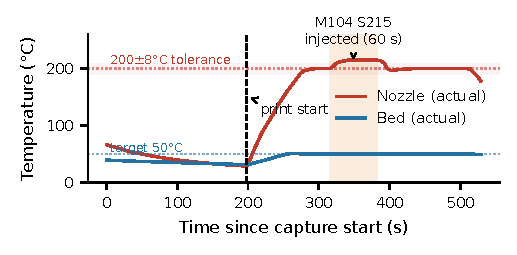
\includegraphics[width=\columnwidth]{fig_thermal_trace}
\caption{Real thermal telemetry from the \icode{cube\_anomaly} run (105
OctoPrint samples, 5\,s interval).  The dashed vertical marks the logged
print-start transition; the shaded orange band marks the 60\,s window in
which \icode{M104 S215} was injected, driving the nozzle (red) out of the
$\pm 8\,^{\circ}$C tolerance band (shaded red) before recovery.  The bed
(blue) holds 50\,$^{\circ}$C throughout.}
\label{fig:thermal}
\end{figure}

%                         --
\subsection{Reputation Propagation (Q2)}
\label{sec:eval_reputation}
%                         --

Each run's rating was submitted on the \icode{quality} dimension against
operator \icode{operator-secnet} via the atomic
\icode{RecordProvenanceWithReputation} invocation.  Starting from the
prior $\mathrm{Beta}(2.0, 2.0)$, the first (f4u2) submission of $r=0.52$
with rater weight $w=0.657$ moved the posterior to
$\mathrm{Beta}(2.34, 2.0)$, i.e.\ score $0.539$ with 95\% Wilson interval
$[0.179, 0.863]$.  Because every subsequent rating exceeded $0.5$, the
$\beta$ pseudocount stayed at $2.0$ and the score rose monotonically as
evidence accumulated.  After all five committed events
(\icode{totalEvents}~$=5$) the on-chain posterior is
$\mathrm{Beta}(4.95, 2.0)$: \textbf{score $0.712$}, 95\% Wilson interval
$[0.356, 0.917]$.

Figure~\ref{fig:beta} plots this measured trajectory.  Two properties
matter.  First, no single print dominates: one mediocre run neither
condemns nor absolves the operator, the intended Bayesian behavior.
Second, the interval tightens as evidence accumulates---its width shrinks
from \textbf{0.684 at $n{=}1$ to 0.561 at $n{=}5$}---so the
confidence-interval gate becomes progressively easier to clear with
attested history and \emph{absence} of history has consequences, closing
the selective-reporting loophole of Section~\ref{sec:boundary}.  Five jobs
is still early in the curve; the trend, not the absolute width, is the
result.

\begin{figure}[t]
\centering
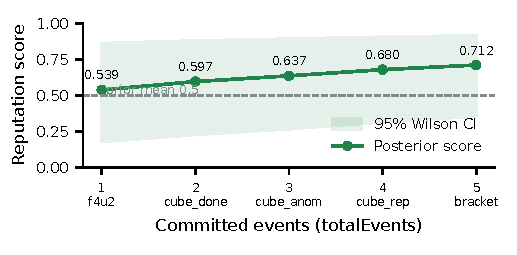
\includegraphics[width=\columnwidth]{fig_beta_posterior}
\caption{Measured on-chain reputation evolution for \icode{operator-secnet}
(quality dimension) across the five committed events.  The score rises
$0.539 \rightarrow 0.712$ and the 95\% Wilson interval (shaded) tightens
from width $0.684$ to $0.561$ as attested evidence accumulates.  Values are
read directly from the ledger after each submission.}
\label{fig:beta}
\end{figure}

%                         --
\subsection{Tamper Detection (Q3)}
\label{sec:eval_tamper}
%                         --

To exercise the post-hoc-tampering row of Table~\ref{tab:taxonomy}, a
single observed nozzle sample in a stored bundle was altered to
235\,$^{\circ}$C.  Verification against the ledger then fails twice,
independently: the recomputed bundle hash no longer matches the on-chain
\icode{offChainDataHash} (Eq.~\eqref{eq:och}), and the Ed25519 signature
over the canonical payload is invalid.  The redundancy matters: detection
survives either a compromised ledger view (signature still fails) or a
leaked device key used to re-sign altered evidence (the ledger hash still
mismatches, because the commitment covers the original signature).  Only
an adversary who can both re-sign \emph{and} rewrite committed Fabric
state---defeat the endorsement policy---evades both checks.

%                         --
\subsection{Latency and Storage Cost (Q4)}
\label{sec:eval_cost}
%                         --

\textbf{Bridge latency (Q4a).}  We instrumented each pipeline stage and
timed it over 100 iterations on each of the four PLA-profile runs
(cube\,$\times$3, bracket).  Figure~\ref{fig:cost}a reports the per-stage
mean with a P95 cap.  The full attest pipeline---parse, payload assembly,
canonicalization, Ed25519 signing, and hash derivation---completes in a
\textbf{0.91\,ms mean}; adding independent verification (signature plus
hash recompute) brings the round trip to \textbf{1.55\,ms}.  Signing
(0.32\,ms) and verification (0.63\,ms) dominate, as expected for Ed25519
over a $\sim$13\,kB payload.  This bridge-side cost is negligible beside
the ledger commit: prior chaincode-side measurement put the atomic
provenance+reputation write at 53.6\,ms mean on the same-host
testbed~\cite{anonymous2026unified}, so the attestation layer adds under
3\% to end-to-end latency.  G-code parsing is the one size-dependent stage:
0.08\,ms for the $\sim$20--38\,kB cube/bracket files but 11.4\,ms for the
5\,MB \icode{f4u2.gcode}---parse scales with design size while signing does
not, because signing covers the fixed-size hash, not the raw G-code.

\textbf{Bundle-size scaling (Q4b).}  Canonical bundle size grows with the
number of retained telemetry samples---from 7.2\,kB (56 samples) to
13.5\,kB (115 samples) across the five runs (Figure~\ref{fig:cost}b)---but
the \textbf{on-chain footprint is a constant 369\,B} (a 32-byte evidence
hash plus the $\sim$337\,B structured record), independent of bundle size.
Compression of the off-chain bundle to its on-chain commitment ranges
19.5$\times$--36.7$\times$.  Linear extrapolation of the per-sample growth
suggests multi-hour prints at 5\,s sampling reach low-single-digit MB
off-chain while the ledger cost stays fixed, motivating the
windowed-summary policies discussed in Section~\ref{sec:discussion}; the
on-chain side already scales independently of print duration.

\begin{figure}[t]
\centering
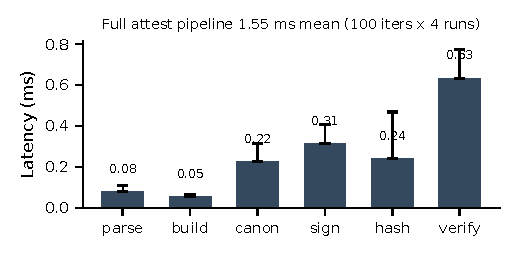
\includegraphics[width=0.49\columnwidth]{fig_bridge_latency}\hfill
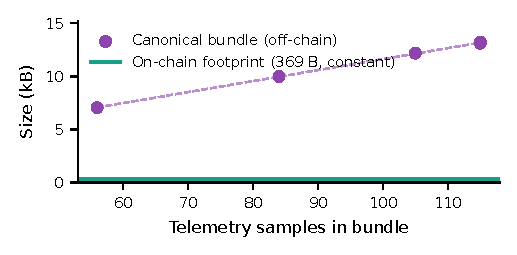
\includegraphics[width=0.49\columnwidth]{fig_bundle_scaling}
\caption{Measured costs.  (a)~Per-stage bridge latency (mean bar, cap at
P95), averaged over 100 iterations on each of the four PLA-profile runs;
the full pipeline incl.\ verification is 1.55\,ms.  (b)~Canonical
off-chain bundle size versus retained samples (five runs); the on-chain
footprint (green) is constant at 369\,B.}
\label{fig:cost}
\end{figure}
